\subsection{UC7 - Ricerca documentale}
\begin{itemize}
    \item \textbf{Identificativo}: UC7
    \item \textbf{Nome}: ricerca documentale
    \item \textbf{Descrione grafica}:
\end{itemize}
\begin{center}
    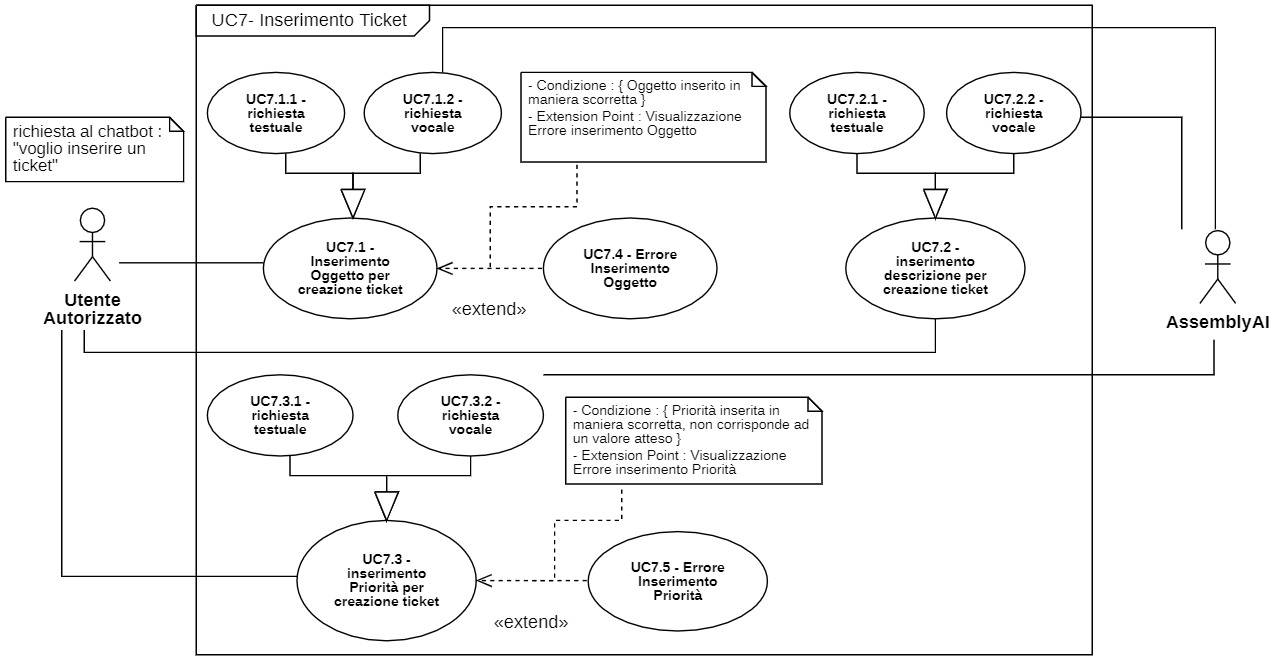
\includegraphics{images/UC7.png} 
\end{center}
 \begin{itemize}
    \item \textbf{Attori}
 \begin{itemize} 
    \item \textit{Primari}: utente autorizzato
    \item \textit{Secondari}: non presenti
 \end{itemize}
 \item \textbf{Precondizione}: l'utente è autorizzato e si trova nell'interfaccia del chatbot.
 \item \textbf{Postcondizione}: il chatbot risponde alla richiesta dell'utente mostrando i documenti trovati.
 \item \textbf{Scenario principale}: l'utente autorizzato chiede al chatbot la ricerca di documenti, specificando il progetto al quale è associato (UC7.1) e il nome del documento (UC7.2).
 \item \textbf{Estensioni}: 
 \begin{itemize} 
    \item il chatbot comunica all'utente che l'azione non è andata a buon fine (UC10).
    \item il chatbot comunica all'utente che non è stato in grado di interpretare il comando (UC2).
    \item il chatbot comunica all'utente che l'inserimento del nome del progetto (UC7.3) o del nome del documento (UC7.4) non sono corretti.
 \end{itemize}
\end{itemize}
\newpage
\subsubsection{UC7.1 - Inserimento progetto}
\begin{itemize}
    \item \textbf{Identificativo}: UC7.1
    \item \textbf{Nome}: inserimento progetto
    \item \textbf{Descrione grafica}: (approfondita in UC7)
    \item \textbf{Attori}
 \begin{itemize} 
    \item \textit{Primari}: utente autorizzato
    \item \textit{Secondari}: non presenti
 \end{itemize}
 \item \textbf{Precondizione}: l'utente ha richiesto al chatbot la ricerca di un documento.
 \item \textbf{Postcondizione}:  l'utente ha comunicato al chatbot il progetto nel quale ricercare i documenti.
 \item \textbf{Scenario principale}: il chatbot chiede all'utente di specificare il progetto nel quale ricercare i documenti. L'utente comunica al chatbot il progetto tramite messaggio testuale (UC7.1.1) o vocale (UC7.1.2).
 \item \textbf{Estensioni}: 
 \begin{itemize} 
    \item il chatbot comunica all'utente che il nome del progetto inserito non è corretto (UC7.3).
 \end{itemize}
\end{itemize}
\subsubsection{UC7.2 - Inserimento nome documento}
\begin{itemize}
    \item \textbf{Identificativo}: UC7.2
    \item \textbf{Nome}: inserimento nome documento
    \item \textbf{Descrione grafica}: (approfondita in UC7)
    \item \textbf{Attori}
 \begin{itemize} 
    \item \textit{Primari}: utente autorizzato
    \item \textit{Secondari}: non presenti
 \end{itemize}
 \item \textbf{Precondizione}: l'utente ha richiesto al chatbot la ricerca di un documento.
 \item \textbf{Postcondizione}:  l'utente ha comunicato al chatbot il nome del documento da ricercare.
 \item \textbf{Scenario principale}: il chatbot chiede all'utente di specificare il nome del documento da ricercare. L'utente comunica al chatbot il nome del documento tramite messaggio testuale (UC7.1.1) o vocale (UC7.1.2).
 \item \textbf{Estensioni}: 
\begin{itemize} 
    \item il chatbot comunica all'utente che il nome del documento inserito non è corretto (UC7.4).
 \end{itemize}
\end{itemize}
\subsubsection{UC7.3 - Errore inserimento nome progetto}
\begin{itemize}
    \item \textbf{Identificativo}: UC7.3
    \item \textbf{Nome}: errore inserimento nome progetto
    \item \textbf{Descrione grafica}: (approfondita in UC7)
    \item \textbf{Attori}
 \begin{itemize} 
    \item \textit{Primari}: utente autorizzato
    \item \textit{Secondari}: non presenti
 \end{itemize}
 \item \textbf{Precondizione}: l'utente ha inserito un nome di progetto non valido.
 \item \textbf{Postcondizione}:  il chatbot comunica all'utente che il nome di progetto specificato non è corretto
 \item \textbf{Scenario principale}: il chatbot comunica all'utente l'errore nell'inserimento del nome di progetto e chiede di reinserirlo.
\end{itemize}
\subsubsection{UC7.4 - Errore inserimento nome documento}
\begin{itemize}
    \item \textbf{Identificativo}: UC7.4
    \item \textbf{Nome}: errore inserimento nome documento
    \item \textbf{Descrione grafica}: (approfondita in UC7)
    \item \textbf{Attori}
 \begin{itemize} 
    \item \textit{Primari}: utente autorizzato
    \item \textit{Secondari}: non presenti
 \end{itemize}
 \item \textbf{Precondizione}: l'utente ha inserito un nome documento non valido.
 \item \textbf{Postcondizione}:  il chatbot comunica all'utente che il nome del documento specificato non è corretto
 \item \textbf{Scenario principale}: il chatbot comunica all'utente l'errore nell'inserimento del nome del documento e chiede di reinserirlo.
\end{itemize}
\newpage